\documentclass[twoside,b5paper,10pt]{article}
\usepackage{AUTstyle}


\title{Paper Template for AACS Workshop }
\author{First Author \and Second Author}

\institution{Department of Automation and Applied Informatics \\
Budapest University of Technology and Economics}

\email{\{aacs,second.author\}@aut.bme.hu}

\headerTitle{Paper Template for AACS \dots}
\headerAuthor{First Author and Second Author}



\begin{document}
\makeAutStyleTitle


\begin{abstract}
Use the \verb|\title|, \verb|\author|, \verb|\institution| and
\verb|\email| commands for providing author information.
Use \verb|\headerTitle| and \verb|\headerAuthor| for providing the short form of the title and author, that will appear on the header of the pages. Please take care having only one header row. When for this reason the title has to be truncated, use \verb|\dots| at the end of the truncated title. When the paper has more than $2$ authors, then provide only the first author in \verb|\headerAuthor| and append ``et al.'' after it.
Use the abstract environment for creating the abstract section. The length
of the abstract must be between $100$ and $150$ words. There are two
categories of the papers that can be submitted. The length of full
papers must between $8$ and $12$ pages, the length of short papers must
be at least $6$ pages.
\end{abstract}


\begin{keywords}
Tutorial; Template; AACS Workhsop; (list of $5$-$7$ keywords in this
format)
\end{keywords}

\section{Introduction}
\label{sec:Introdu}

Authors of the AACS Workhsop are encouraged to create their papers
to the workshop in \LaTeX \ using the style file provided at
www.aut.bme.hu$\slash$aacs.

Use the \verb|\title|, \verb|\author|, \verb|\institution| and
\verb|\email| commands for providing author information.
Use \verb|\headerTitle| and \verb|\headerAuthor| for providing the short form of the title and author, that will appear on the header of the pages. Please take care having only one header row. When for this reason the title has to be truncated, use \verb|\dots| at the end of the truncated title. When the paper has more than $2$ authors, then provide only the first author in \verb|\headerAuthor| and append ``et al.'' after it.

In this short template, you have some examples how to import
figures, tables into the document, how to write equations, and how
to reference these objects within the text of your paper. The
commands for these operations are not explicitly noted in this text,
but having the \LaTeX \ source file of this template, you can find
it.

The organization of this template is as follows.
\sectionname~\ref{sec:tables-figures} shows how tables and figures can be
inserted into the paper. \sectionname~\ref{sec:Mathema-formula} provides
some example about mathematical formulas. \sectionname~\ref{sec:theorem}
shows how theorem-like environments have to be used, and how you can
typeset algorithms. \sectionname~\ref{sec:bib} shows and example for
citing and inserting bibliography entries into the paper.

\section{Tables and Figures}
\label{sec:tables-figures}

In \LaTeX \ you can work with two types of picture formats, the one
with the extension of .eps and with other type of pictures like
.png, .jpg, .pdf etc. In the first case the output of the source
code is .dvi, and you have to convert it with \emph{dvi2pdf} into
pdf. In the latter case you can directly create pdf files from the
\LaTeX \ source using the \verb|PDFLaTeX| command. \textbf{Please
use .png as your picture extension for the AACS workshop.}

You can insert figures into the text practically in two ways. When
you need more space for a figure, simply insert it as single figure
as shown in \figurename~\ref{fig:simple}.

\begin{figure}[htb]
 \centerline{\includegraphics[width=.85\columnwidth]{.//Figure/BMElogo.png}}
 \caption{The logo of the University}
 \label{fig:simple}
\end{figure}

However because of space saving reasons you can put two figures in
the same row as shown in \figurename~\ref{fig:two}(a) and
\ref{fig:two}(b).
\begin{figure}[htb]
  \vspace{3pt}
  \centerline{
  \hbox{
  \hspace{0.0in}
        \includegraphics[width = 0.45\columnwidth]{Figure/BMElogo.png}
        \hspace{0.1\columnwidth}
        \includegraphics[width=0.45\columnwidth]{Figure/BMElogo.png}
    }
  }
  \vspace{3pt}
  \hbox{\hspace{0.2\columnwidth} (a) \hspace{0.5\columnwidth} (b)}
  \caption{ (a) BME logo 1 (b) BME logo 2}
  \label{fig:two}
\end{figure}


You can also use the \textbf{subfloat} package for arranging your figures. In this case, you can easily reference only the part of the whole figure. For example \figurename~\ref{subfig:one} is the first part of the \figurename~\ref{fig:bme}.

 \begin{figure}[h]
        \centering
%%----start of first subfigure----
        \subfloat[The first figure]{
            \label{subfig:one} %% label for first subfigure
            \includegraphics[width=0.4\linewidth]{Figure/BMElogo.png}}
        \hspace{0.02\linewidth}
%%----start of second subfigure----
        \subfloat[The second figure]{
            \label{subfig:two} %% label for second subfigure
            \includegraphics[width=0.4\linewidth]{Figure/BMElogo.png}}
        \caption{Some logo of the BME}
        \label{fig:bme} %% label for entire figure
\end{figure}




For the camera ready manuscript you have to
provide the source code of your \LaTeX \ work (.tex file, the
figures and the .bib files compressed (zip)).

You can create tables as shown in \tablename~\ref{tab:first}. Please
insert the caption of the table above the table by placing the
caption just after the \verb|\begin{table}| command.

\begin{table}[htb]
\caption{Sample table using the different Greek letters}
\begin{center}
\begin{tabular}{|c|c|}
\hline
\textbf{Command} & \textbf{Appearance} \\
\hline
\verb|$\alpha$| & $\alpha$ \\
\hline
\verb|$\beta$| & $\beta$ \\
\hline
\verb|$\Gamma$| & $\Gamma$ \\
\hline
\verb|$\gamma$| & $\gamma$ \\
\hline
\verb|$\sigma$| & $\sigma$ \\
\hline
\end{tabular}
\end{center}
\label{tab:first}
\end{table}


\section{Mathematical formulas}
\label{sec:Mathema-formula}

In order to obtain a mathematical formula using \LaTeX, you must
enter mathematics mode before the formula and leave it afterwards.
Mathematical formulae can occur either embedded in text (in-line
mode) or else displayed between lines of text. When a formula occurs
within the text of a paragraph one should place a \$ sign before and
after the formula, in order to enter and leave mathematics mode.

For example the command \verb|$\sigma_{min}$| will cause
$\sigma_{min}$ in the text. You can insert more complex formulas as
well, for example: $\sum_{i=1}^{n}i^{2}$ is created by the command
\verb|$\sum_{i=1}^{n}i^{2}$|.

Not in-line equation can be created as shown in
\equationname~\eqref{eq:sum}. In case of not in-line equations please
always use numbered equations.
\begin{equation}
S=\sum_{i=1}^{n}\alpha*i^2 \label{eq:sum}
\end{equation}

When you want to write more equations in succession you can do this
as shown in \equationname~\eqref{eq:array}.


%\begin{eqnarray}
%4x-1 &=& 2x+4 \\
%2x-1 &=& 4 \\
%2x &=& 5 \\
%x &=&  \frac{5}{2}
%\end{eqnarray}

\begin{eqnarray}
  \label{eq:array}
4x-1 &=& 2x+4 \nonumber \\
2x-1 &=& 4 \\
2x &=& 5 \nonumber \\
 x &=&  \frac{5}{2} \nonumber
\end{eqnarray}

A more complex equation can be seen in \equationname
~\ref{equ:complex}.

\begin{equation}
 \label{equ:complex}
f(x) = \left\{ {
\begin{array}{*{20}l}
   {1\ \mbox{if} \ x \in A}  \\
   {0\ \mbox{otherwise}\,}  \\
\end{array}} \right.
\end{equation}

\textbf{Take care of using} \verb|\eqref| \textbf{when referencing the number of an equation.}

\section{Theorem environments}
\label{sec:theorem}

 You can use several theorem-like environments
that are defined in the style file. For the proofs use
\verb|\begin{proof}| and \verb|\end{proof}| commands.

\begin{definition}
This is a definition. The typesetting of the definition is
predefined in the style file. The numbering of the different
theorem-like environments are continuous.
\end{definition}


\begin{theorem}
\label{th:first} This is the first theorem of the paper.
\end{theorem}

\begin{proof}
This is the proof of Theorem~\ref{th:first}
\end{proof}


You can use the environments shown in \tablename~\ref{tab:env}.

\begin{table}[htb]
\caption{Different environments}
\label{tab:env}
\begin{center}
\begin{tabular}{|r | l|}
 \hline
 Environment name & Appearing text \\
 \hline
 theorem & Theorem \\
 cor & Corollary \\
 lemma & Lemma \\
 claim & Claim \\
 axiom & Axiom \\
 conj & Conjecture \\
 fact & Fact \\
 hypo & Hypothesis \\
 assumption & Assumption \\
 proposition & Proposition \\
 crit & Criterion \\
 definition & Definition \\
 example & Example \\
 remark & Remark \\
 problem & Problem \\
 prin & Principle \\
 alg & Algorithm \\
\hline
\end{tabular}
\end{center}
\end{table}

When you want to typeset the pseudocode of an algorithm you can use
the Algorithm environment as shown in Algorithm~\ref{alg:alg}.

\begin{algorithm}
  \caption{Pseudo code of the Apriori algorithm}
\begin{algorithmic}[1]
\label{alg:alg}
 \STATE \textbf{procedure} Apriori($\sigma_{min}$)
 \STATE $L^{1}$ = find frequent $1$-itemsets
 \FOR{$k = 2$;$L^{k-1}$ $!=$ $null$;$k$++}
 \STATE $C^{k}$ = AprioriGen($L^{k-1}$)
 \FORALL {transaction $t \in D_{I}$}
 \STATE $C^{t} = subset(C^{k},t)$
 \FORALL {candidate $c$ in $C^{t}$ }
 \STATE $c$.counter++
 \FORALL {$c$ in $C^{k}$}
 \IF{ $c$.counter $>$ $\sigma_{min}$}
 \STATE $L^{k}.Add(c)$
 \ENDIF
 \ENDFOR
 \ENDFOR
 \ENDFOR
 \ENDFOR
 \STATE \textbf{return} $C^{k}$

\end{algorithmic}
\end{algorithm}


\section{Bibliography}
\label{sec:bib}

You have to use the \verb|\makeAutBib| command for your
bibliography. The input parameter of the command is the comma
separated list of bib files without the extension. You can also find
a sample bib file on the Workshop's web site where also the style
file and this sample \LaTeX \ template are provided. You can cite
any of the entries of the bib files for example ~\cite{ han00mining}
or ~\cite{burdick01mafia}. The advantage of using bib files is that
only those bibliographies will appear in the References section that
are cited in the text \cite{proba}.

If you have any question related to writing your \LaTeX \ paper
please contact the chair of the conference(e-mail: aacs@aut.bme.hu).

You can submit your paper via the web page of the conference. The
submission of the papers will be opened soon.

\section*{Acknowledgments}
 { \small The author would like to express his thanks to Istv�n Vajk~\footnote{Please mention the name of your advisor in the
Acknowledgements section. } for his support as a scientific advisor.
This work has been supported by the \dots \footnote{Please mention
the institution or organization that has supported your research
work.} }

\makeAutBib{reni,itemsetmining}

\end{document}
